\documentclass{article}
\usepackage{graphicx}
\usepackage{amsmath}
\usepackage[parfill]{parskip}
\usepackage{hyperref}
\usepackage{tikz}
\usepackage{biblatex}
\addbibresource{references.bib}
\graphicspath{ {./figures/} }

\title{COMP.SEC.220 Security Protocol\footnote{github --- \url{https://github.com/ancuongnguyen07/SecurityProtocol}}}
\author{Cuong Nguyen --- LAB 4}
\date{22/09/2022}

\begin{document}
    
\maketitle

\section*{Exercise 1}

\subsection*{Task 1}
%
\begin{itemize}
    \item Alice sends Bob \(A = g^{a} \mod p: 4 = 7^{6} \mod 11\)
    \item Bobs sends Alice \(B = g^{a} \mod p: 8 = 7^{9}  \mod 11\)
    \item Alice computes \(s = B^{a} \mod p: 3 = 8^{6} \mod 11\)
    \item Bobs computes \(s = A^{b} \mod p: 3 = 4^{9} \mod 11\)
    \item Now Bobs and Alice share the final key \(s = 3\)
\end{itemize}

\subsection*{Task 2 + 3}
%
Because g = 5 is the primitive root of p = 47, we can solve \(Y = g^{b}
\mod p\ or\ 3 = 5^{b} \mod 47\) in 46 trials. Running a simple for-loop,
I found that the value of \emph{b} is 20. So the shared key is:
\begin{align*}
    s &= X^{b} \mod p \\
    2 &= 38^{20} \mod 47
\end{align*}
After running the Caesar decryption script with shift key 2, I obtained:
\begin{center}
    \textbf{YOU HAVE REACHED A NEW LEVEL --- ADMIN}
\end{center}

\section*{Exercise 2}
%

%%%%%% ROUND 1
\tikzset{every picture/.style={line width=0.75pt}} %set default line width to 0.75pt        

\begin{figure}[!hpt]
    \centering
    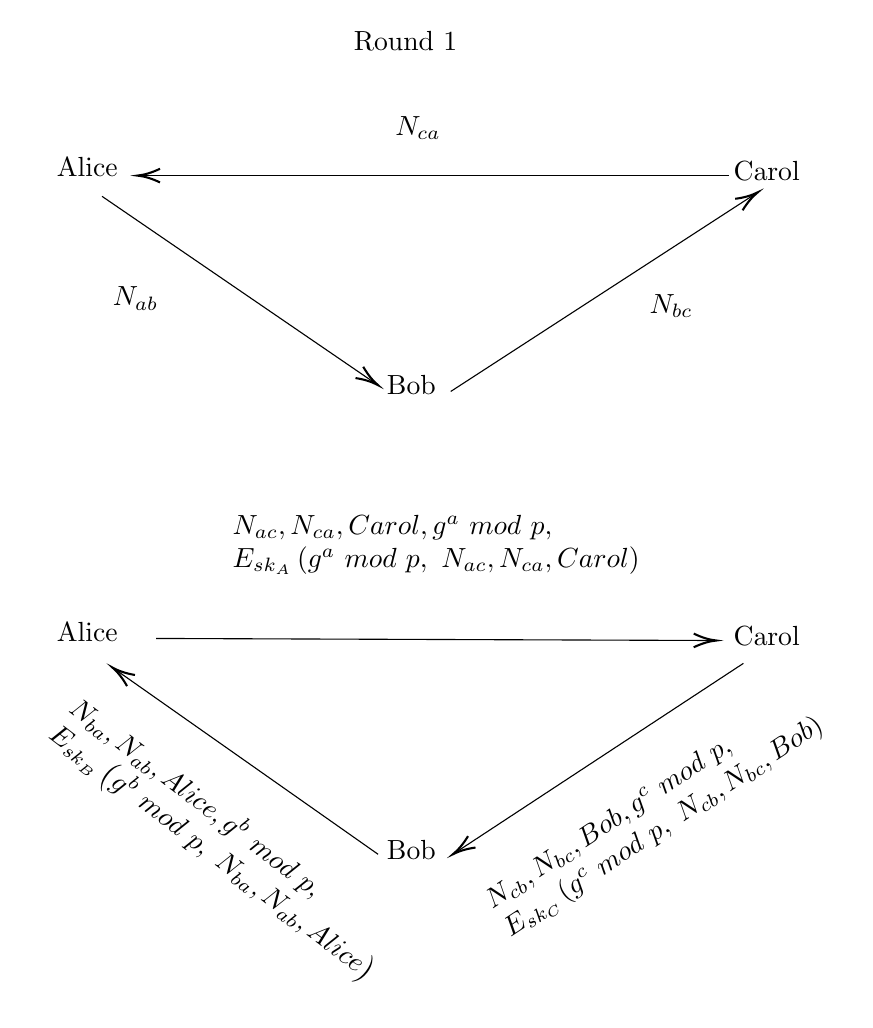
\begin{tikzpicture}[x=0.75pt,y=0.75pt,yscale=-1,xscale=1]
        %uncomment if require: \path (0,585); %set diagram left start at 0, and has height of 585
        
        %Straight Lines [id:da3334516865831303] 
        \draw    (471,81) -- (188,81) ;
        \draw [shift={(186,81)}, rotate = 360] [color={rgb, 255:red, 0; green, 0; blue, 0 }  ][line width=0.75]    (10.93,-3.29) .. controls (6.95,-1.4) and (3.31,-0.3) .. (0,0) .. controls (3.31,0.3) and (6.95,1.4) .. (10.93,3.29)   ;
        %Straight Lines [id:da94114870161733] 
        \draw    (169,91) -- (300.35,180.87) ;
        \draw [shift={(302,182)}, rotate = 214.38] [color={rgb, 255:red, 0; green, 0; blue, 0 }  ][line width=0.75]    (10.93,-3.29) .. controls (6.95,-1.4) and (3.31,-0.3) .. (0,0) .. controls (3.31,0.3) and (6.95,1.4) .. (10.93,3.29)   ;
        %Straight Lines [id:da0011322007155480929] 
        \draw    (337,185) -- (483.32,90.09) ;
        \draw [shift={(485,89)}, rotate = 147.03] [color={rgb, 255:red, 0; green, 0; blue, 0 }  ][line width=0.75]    (10.93,-3.29) .. controls (6.95,-1.4) and (3.31,-0.3) .. (0,0) .. controls (3.31,0.3) and (6.95,1.4) .. (10.93,3.29)   ;
        %Straight Lines [id:da5968740748299537] 
        \draw    (195,304) -- (463,304.99) ;
        \draw [shift={(465,305)}, rotate = 180.21] [color={rgb, 255:red, 0; green, 0; blue, 0 }  ][line width=0.75]    (10.93,-3.29) .. controls (6.95,-1.4) and (3.31,-0.3) .. (0,0) .. controls (3.31,0.3) and (6.95,1.4) .. (10.93,3.29)   ;
        %Straight Lines [id:da04098198791931473] 
        \draw    (302,408) -- (175.64,319.15) ;
        \draw [shift={(174,318)}, rotate = 35.11] [color={rgb, 255:red, 0; green, 0; blue, 0 }  ][line width=0.75]    (10.93,-3.29) .. controls (6.95,-1.4) and (3.31,-0.3) .. (0,0) .. controls (3.31,0.3) and (6.95,1.4) .. (10.93,3.29)   ;
        %Straight Lines [id:da8644686811967816] 
        \draw    (478,316) -- (339.67,406.9) ;
        \draw [shift={(338,408)}, rotate = 326.69] [color={rgb, 255:red, 0; green, 0; blue, 0 }  ][line width=0.75]    (10.93,-3.29) .. controls (6.95,-1.4) and (3.31,-0.3) .. (0,0) .. controls (3.31,0.3) and (6.95,1.4) .. (10.93,3.29)   ;
        
        % Text Node
        \draw (146,71) node [anchor=north west][inner sep=0.75pt]   [align=left] {Alice};
        % Text Node
        \draw (305,176) node [anchor=north west][inner sep=0.75pt]   [align=left] {Bob};
        % Text Node
        \draw (472,73) node [anchor=north west][inner sep=0.75pt]   [align=left] {Carol};
        % Text Node
        \draw (309,51.4) node [anchor=north west][inner sep=0.75pt]    {$N_{ca}$};
        % Text Node
        \draw (173,133.4) node [anchor=north west][inner sep=0.75pt]    {$N_{ab}$};
        % Text Node
        \draw (431.5,136.9) node [anchor=north west][inner sep=0.75pt]    {$N_{bc}$};
        % Text Node
        \draw (146,295) node [anchor=north west][inner sep=0.75pt]   [align=left] {Alice};
        % Text Node
        \draw (305,400) node [anchor=north west][inner sep=0.75pt]   [align=left] {Bob};
        % Text Node
        \draw (472,297) node [anchor=north west][inner sep=0.75pt]   [align=left] {Carol};
        % Text Node
        \draw (224,241.4) node [anchor=north west][inner sep=0.75pt]    {$ \begin{array}{l}
        N_{ac} ,N_{ca} ,Carol,g^{a} \ mod\ p,\\
        E_{sk_{A}}\left( g^{a} \ mod\ p,\ N_{ac} ,N_{ca} ,Carol\right)
        \end{array}$};
        % Text Node
        \draw (153.86,324.31) node [anchor=north west][inner sep=0.75pt]  [rotate=-37.28]  {$ \begin{array}{l}
        N_{ba} ,N_{ab} ,Alice,g^{b} \ mod\ p,\\
        E_{sk_{B}}\left( g^{b} \ mod\ p,\ N_{ba} ,N_{ab} ,Alice\right)
        \end{array}$};
        % Text Node
        \draw (343.56,428.56) node [anchor=north west][inner sep=0.75pt]  [rotate=-326.46]  {$ \begin{array}{l}
        N_{cb} ,N_{bc} ,Bob,g^{c} \ mod\ p,\\
        E_{sk_{C}}\left( g^{c} \ mod\ p,\ N_{cb} ,N_{bc} ,Bob\right)
        \end{array}$};
        % Text Node
        \draw (289,10) node [anchor=north west][inner sep=0.75pt]   [align=left] {Round 1};
        
        
    \end{tikzpicture}
        
\end{figure}


%%%%%% ROUND 2
\tikzset{every picture/.style={line width=0.75pt}} %set default line width to 0.75pt        

\begin{figure}[!hpt]
    \centering
    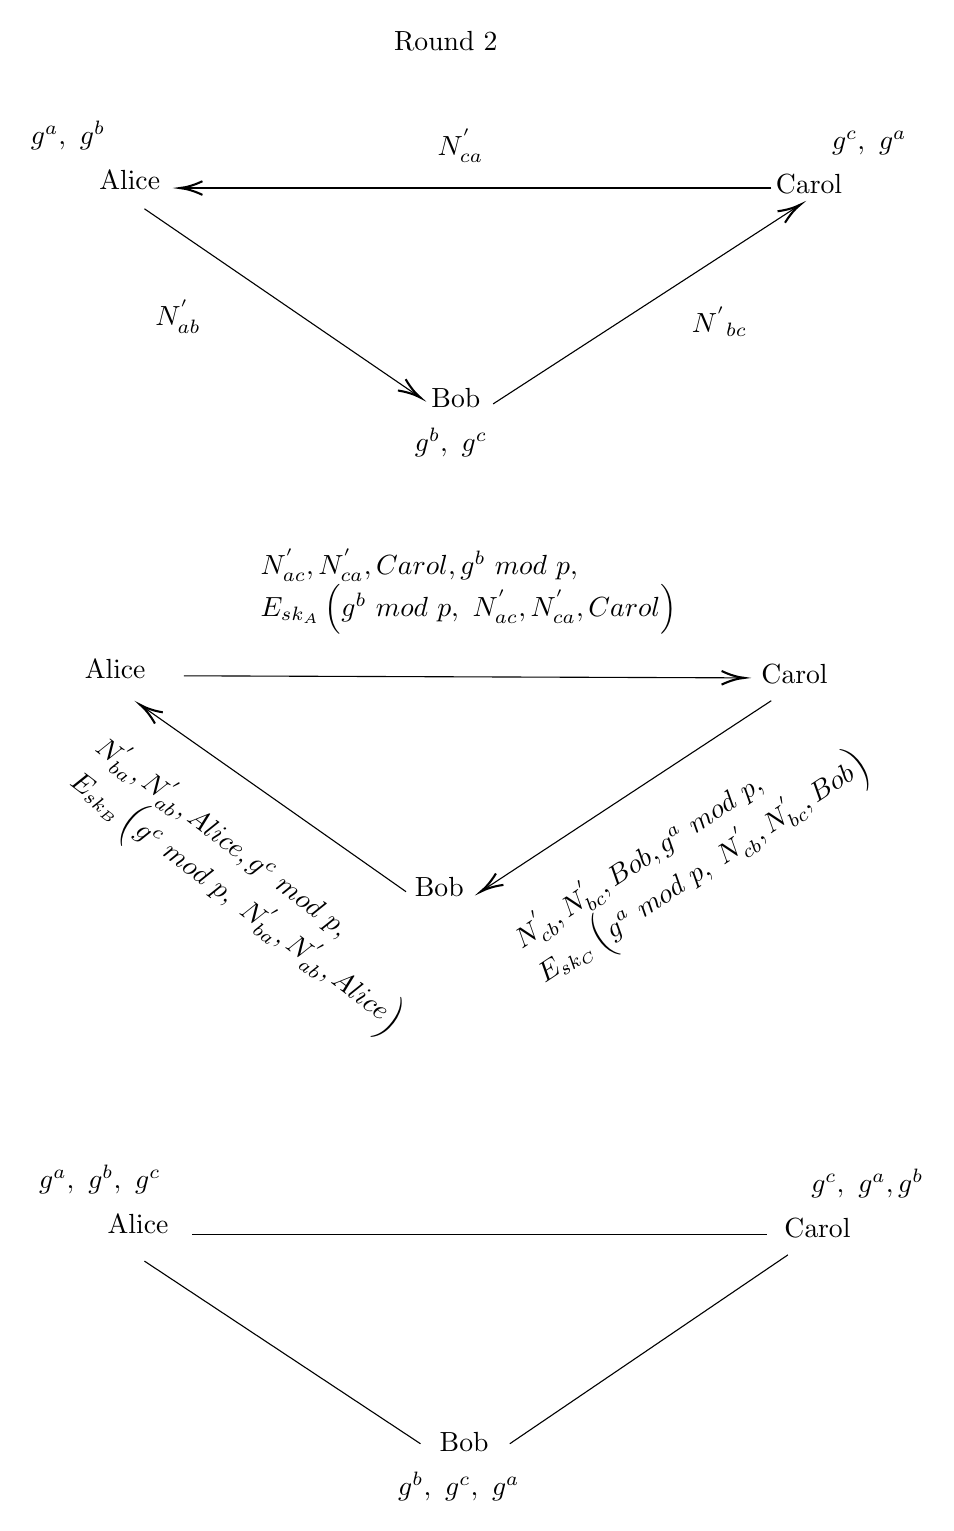
\begin{tikzpicture}[x=0.75pt,y=0.75pt,yscale=-1,xscale=1]
        %uncomment if require: \path (0,769); %set diagram left start at 0, and has height of 769
        
        %Straight Lines [id:da8541968213607035] 
        \draw    (479,96) -- (196,96) ;
        \draw [shift={(194,96)}, rotate = 360] [color={rgb, 255:red, 0; green, 0; blue, 0 }  ][line width=0.75]    (10.93,-3.29) .. controls (6.95,-1.4) and (3.31,-0.3) .. (0,0) .. controls (3.31,0.3) and (6.95,1.4) .. (10.93,3.29)   ;
        %Straight Lines [id:da1237435555212254] 
        \draw    (177,106) -- (308.35,195.87) ;
        \draw [shift={(310,197)}, rotate = 214.38] [color={rgb, 255:red, 0; green, 0; blue, 0 }  ][line width=0.75]    (10.93,-3.29) .. controls (6.95,-1.4) and (3.31,-0.3) .. (0,0) .. controls (3.31,0.3) and (6.95,1.4) .. (10.93,3.29)   ;
        %Straight Lines [id:da48554882078244543] 
        \draw    (345,200) -- (491.32,105.09) ;
        \draw [shift={(493,104)}, rotate = 147.03] [color={rgb, 255:red, 0; green, 0; blue, 0 }  ][line width=0.75]    (10.93,-3.29) .. controls (6.95,-1.4) and (3.31,-0.3) .. (0,0) .. controls (3.31,0.3) and (6.95,1.4) .. (10.93,3.29)   ;
        %Straight Lines [id:da16447444523978727] 
        \draw    (196,331) -- (464,331.99) ;
        \draw [shift={(466,332)}, rotate = 180.21] [color={rgb, 255:red, 0; green, 0; blue, 0 }  ][line width=0.75]    (10.93,-3.29) .. controls (6.95,-1.4) and (3.31,-0.3) .. (0,0) .. controls (3.31,0.3) and (6.95,1.4) .. (10.93,3.29)   ;
        %Straight Lines [id:da09342465789947885] 
        \draw    (303,435) -- (176.64,346.15) ;
        \draw [shift={(175,345)}, rotate = 35.11] [color={rgb, 255:red, 0; green, 0; blue, 0 }  ][line width=0.75]    (10.93,-3.29) .. controls (6.95,-1.4) and (3.31,-0.3) .. (0,0) .. controls (3.31,0.3) and (6.95,1.4) .. (10.93,3.29)   ;
        %Straight Lines [id:da5299303856965484] 
        \draw    (479,343) -- (340.67,433.9) ;
        \draw [shift={(339,435)}, rotate = 326.69] [color={rgb, 255:red, 0; green, 0; blue, 0 }  ][line width=0.75]    (10.93,-3.29) .. controls (6.95,-1.4) and (3.31,-0.3) .. (0,0) .. controls (3.31,0.3) and (6.95,1.4) .. (10.93,3.29)   ;
        %Straight Lines [id:da47838719409695674] 
        \draw    (200,600) -- (477,600) ;
        %Straight Lines [id:da7171897321272096] 
        \draw    (177,613) -- (310,701) ;
        %Straight Lines [id:da09618867410220122] 
        \draw    (353,701) -- (487,610) ;
        
        % Text Node
        \draw (154,86) node [anchor=north west][inner sep=0.75pt]   [align=left] {Alice};
        % Text Node
        \draw (314,191) node [anchor=north west][inner sep=0.75pt]   [align=left] {Bob};
        % Text Node
        \draw (480,88) node [anchor=north west][inner sep=0.75pt]   [align=left] {Carol};
        % Text Node
        \draw (317,66.4) node [anchor=north west][inner sep=0.75pt]    {$N_{ca}^{'}$};
        % Text Node
        \draw (181,148.4) node [anchor=north west][inner sep=0.75pt]    {$N_{ab}^{'}$};
        % Text Node
        \draw (439.5,151.9) node [anchor=north west][inner sep=0.75pt]    {$N^{'}{}_{bc}$};
        % Text Node
        \draw (147,322) node [anchor=north west][inner sep=0.75pt]   [align=left] {Alice};
        % Text Node
        \draw (306,427) node [anchor=north west][inner sep=0.75pt]   [align=left] {Bob};
        % Text Node
        \draw (473,324) node [anchor=north west][inner sep=0.75pt]   [align=left] {Carol};
        % Text Node
        \draw (225,268.4) node [anchor=north west][inner sep=0.75pt]    {$ \begin{array}{l}
        N_{ac}^{'} ,N_{ca}^{'} ,Carol,g^{b} \ mod\ p,\\
        E_{sk_{A}}\left( g^{b} \ mod\ p,\ N_{ac}^{'} ,N_{ca}^{'} ,Carol\right)
        \end{array}$};
        % Text Node
        \draw (154.86,351.31) node [anchor=north west][inner sep=0.75pt]  [rotate=-37.28]  {$ \begin{array}{l}
        N_{ba}^{'} ,N_{ab}^{'} ,Alice,g^{c} \ mod\ p,\\
        E_{sk_{B}}\left( g^{c} \ mod\ p,\ N_{ba}^{'} ,N_{ab}^{'} ,Alice\right)
        \end{array}$};
        % Text Node
        \draw (344.56,455.56) node [anchor=north west][inner sep=0.75pt]  [rotate=-326.46]  {$ \begin{array}{l}
        N_{cb}^{'} ,N_{bc}^{'} ,Bob,g^{a} \ mod\ p,\\
        E_{sk_{C}}\left( g^{a} \ mod\ p,\ N_{cb}^{'} ,N_{bc}^{'} ,Bob\right)
        \end{array}$};
        % Text Node
        \draw (121,62.4) node [anchor=north west][inner sep=0.75pt]    {$g^{a} ,\ g^{b}$};
        % Text Node
        \draw (507,67.4) node [anchor=north west][inner sep=0.75pt]    {$g^{c} ,\ g^{a}$};
        % Text Node
        \draw (306,210.4) node [anchor=north west][inner sep=0.75pt]    {$g^{b} ,\ g^{c}$};
        % Text Node
        \draw (158,589) node [anchor=north west][inner sep=0.75pt]   [align=left] {Alice};
        % Text Node
        \draw (318,694) node [anchor=north west][inner sep=0.75pt]   [align=left] {Bob};
        % Text Node
        \draw (484,591) node [anchor=north west][inner sep=0.75pt]   [align=left] {Carol};
        % Text Node
        \draw (125,565.4) node [anchor=north west][inner sep=0.75pt]    {$g^{a} ,\ g^{b} ,\ g^{c}$};
        % Text Node
        \draw (497,567.4) node [anchor=north west][inner sep=0.75pt]    {$g^{c} ,\ g^{a} ,g^{b}$};
        % Text Node
        \draw (298,713.4) node [anchor=north west][inner sep=0.75pt]    {$g^{b} ,\ g^{c} ,\ g^{a}$};
        % Text Node
        \draw (296,19) node [anchor=north west][inner sep=0.75pt]   [align=left] {Round 2};
        
    \end{tikzpicture}

    \caption{Authenticated and extended DH key exchange \cite{3_exchange}\cite{course_slides}}
\end{figure}

At final step, the common secret key is \(K = g^{abc} \mod p\)

\section*{Exercise 3}
%
\begin{figure}[!hpt]
    \centering
    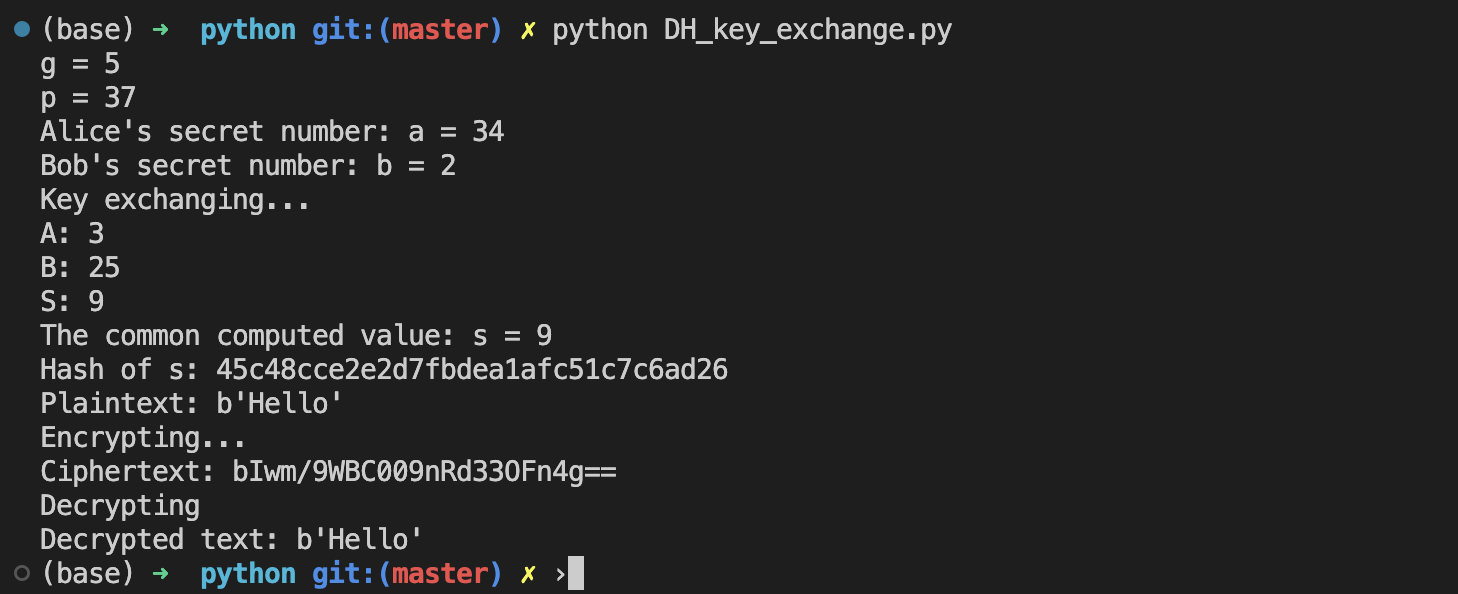
\includegraphics[width=\textwidth, height=\textheight, keepaspectratio]{DH_implementation.png}
    \caption{DH-implementation Python program}
\end{figure}

\textbf{The security of a D-H key exchange protocol is based on?}\\
It's based on the choice of \emph{g} and \emph{p}.

\textbf{The D-H key exchange protocol is vulnerable to?}\\
It is vulnerable to a man-inthe-middle-attack as it doesn't provide
any authentication of the communicating parties.

\textbf{What is the condition for selecting a good value of o in a D-H key exchange protocol?}\\
The order of \emph{p} should have a large prime factor. It is sometimes
calculated as \(p = 2q + 1\), since the order of \emph{p} is then only dvisible
by 2 and \emph{q}\cite{wiki}.

\printbibliography{}

\end{document}